
Two-Level Segregated Fit (TLSF) is a dynamic storage allocator, first introduced by M. Masmano et al.~\cite{TLSF} that is designed to be used in real-time applications. TLSF outperforms other allocators in that it has a bounded and short response time, and a bounded and low fragmentation, making it highly predictable.

The work of the TLSF authors primarily focuses on explicit low-level allocation primitives, with no explicit consideration for garbage collection. Therefore, investigating how TLSF can be adapted to fit into the context of garbage collection represents a crucial and promising avenue for advancing its development.

As the name TLSF implies, the allocator is a free-list based allocator that uses segregated-fit, storing multiple free-lists containing blocks of set size classes. To efficiently lookup what free-list contain blocks, TLSF employs two levels of bitmaps, one bitmap for size classes that are separated by powers of two called first-level, and a second-level that subdivides the first-level size classes linearly. In the reference implementation, the number of first- and second-levels are both limited to 32 in order to fit in 32-bit values. Additionally, the number of second-levels are recommended to be a power of two for efficiency reasons, so that simple bit instructions can be used.

Blocks in the allocator are stored in two doubly-linked list structures, first in a physically ordered list and again in one of the free-lists if the block is free. To facilitate this, each block has an associated header allocated next to it. This header describes both the size of the block but also how it falls withing both of these doubly-linked lists. The difference in representation is shown in Figure~\ref{fig:blockheader_reference}, where free blocks store more data than allocated blocks. Additionally, block sizes are always aligned to a multiple of eight (the allocation unit is 8 bytes for 64-bit architecture), the least significant three bits can be used to store metadata about the block, however only the least two are used. The bits store information about whether the block is busy or free (F-bit) and whether the block is the last one of the pool (T-bit), as also shown in Figure~\ref{fig:blockheader_reference}.

% TODO: Fix correct citation for figure?
\begin{figure}[H]
    \centering
    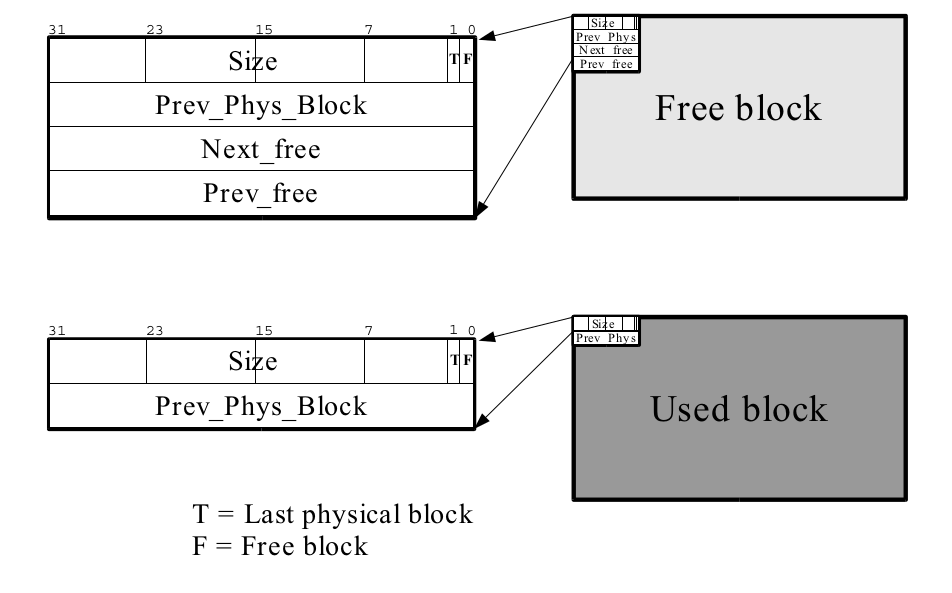
\includegraphics[width=0.65\textwidth]{figures/blockheader_reference.png}
    \caption{Representation of free and allocated block headers in 32-bit architecture. For a 64-bit architecture, each individual field is 8 bytes instead of 4 bytes. (Taken from~\cite{TLSF}).}
    \label{fig:blockheader_reference}
\end{figure}

\subsubsection{Allocation and Freeing Strategy}

From the user's perspective, TLSF behaves identically to how the malloc/free API~\cite{malloc_free} does in libc for example. However, its inner workings is what makes it unique and different from other allocators.

When a user requests N number of bytes from the allocator, N is aligned to any needed alignment and padding before a block of the desired size is searched for. If a block of the specific range that the size falls within is not found, the allocator tries to look for a block that is larger than the desired size. If multiple blocks are present in any of the free-lists the allocator decides to take a block from, the first block is chosen. This policy is sometimes referred to as Good-Fit, a combination of best- and first-fit. Additionally, if a larger block is found, it is split up into two blocks, one of which is returned to the user, and another that is inserted back into the allocator. 

When a user requests N bytes from the allocator, the allocator aligns N to meet any necessary alignment requirements and applies padding. Subsequently, it searches for a block matching the desired size. If no block within the specific size range is found, the allocator continues its search to identify a larger block. If no block is found, a NULL value is returned. However, if a list containing blocks is found, the allocator picks the first block in the list, regardless of the number of blocks in it. The policy of searching for free-lists and choosing the first block is called Good-Fit by the authors, referred to as a combination of best- and first-fit. Moreover, if a larger block is located, the allocator divides it into two blocks. One block is allocated to the user, and the other is reintegrated back into the allocator.

Later on, when a user decides to free an allocated block it is implicitly attempted to be coalesced, or merged, with its physical neighbors. The reason for coalescing immediately when freeing is to be able to have larger blocks available for larger requests sizes as often as possible.


%%% Local Variables:
%%% mode: latex
%%% TeX-master: "main"
%%% End:
